% to-do
% Add more to introduction, explain more about general binaries the process of how it works
% 
% add more regarding common binaries

% Captions on all graphics

% xray accretion section

% maybe add xray binary type sections? to cover hmxbs and lmxbs

% good excerpt on CEE evololution over time
%As mentioned before, the common envelope evolution (CEE) has been first proposed in 1976 to account for the origin of cataclysmic variables (CVs). CVs are binaries consisting of a WD with a typical mass of around and an MS companion star with a typical mass of , in which the MS star fills its Roche lobe and undergoes the mass transfer. They typically have an orbital period of 1 to 10 h. Regarding the origin of CV systems, the question is how to form such massive WDs in such a close binary system with an orbital period of a few hours. According to the stellar evolution theory, massive WDs could be formed from cores of red giants (or supergiants) before their envelopes are removed. In this case, the orbital period of a binary system needs to be long enough to keep the red giant (or supergiant) within its Roche lobes until a massive core is formed. Then, a mechanism is needed to drastically reduce the orbital period to a few hours consequently to match the observed periods of CVs. This therefore leads to the proposal of CEE (e.g. [198], [223], [224]). By adopting the CE scenario, the origin of V 471 Tau was successfully explained [198], i.e., a detached binary in the Hyades cluster which has a WD and a K-type dwarf, with an orbital period of . This binary system is expected to evolve into a CV system within a few yr.


% Add section explaining what causes binaries to draw closer to eachother, why its needed, etc etc, 

% GwR, Mass Loss, and Magnetic braking

%

%
\documentclass[12pt, letterpaper]{article}
\usepackage{titlesec}
\usepackage{graphicx}
\usepackage{geometry}
\usepackage{abstract}
\usepackage[T1]{fontenc}
\usepackage{lipsum}
\usepackage{tabularx}
\usepackage[sorting=none, style=nature]{biblatex} 
\usepackage[labelfont=bf, labelsep=colon, textfont=it]{caption}


\renewcommand{\abstractnamefont}{\normalfont\Large\bfseries} 

\titleformat{\section}
  {\normalfont\Large\bfseries\centering} % Formatting for the section title
  {} % Empty label (hides the number)
  {0pt} % No spacing before title
  {} % No additional formatting

\titleformat{\subsection}
    {\normalfont\Large\bfseries\centering}
    {\thesubsection}
    {.5em}
    {}
\titleformat{\subsubsection}
    {\normalfont\small\bfseries\centering}
    {\thesubsubsection}
    {.5em}
    {}


\addbibresource{sources.bib} %Import the bibliography file
\title{Mass Transfer in Binary Star Evolution}
\author{Pierson Lipschultz\thanks{Mentored by Joseph DalSanto}}

\date{\today}
\begin{document}
\maketitle
\begin{abstract}
    \normalsize
    In this paper, I will investigate the properties of mass transfer in binary stars, including the Roche Lobe model, evolutionary stages, evolution, rate, progenitors, and resultant stars. I will use the Roche Lobe model to catalyze the stars into Detached (Wind Accretion), Roche Lobe Overflow (RLO), and Contact Binaries (CB). I will then look at stars that fit these stages and investigate them further using data from example systems corroborated with data from POSYDON.

    I found that ... and ...
\end{abstract}

\pagebreak

\section{\centering Introduction} % amaybe include a section on x-ray emission???

    Most of the stars we see in the night sky are not actually single stars, instead consisting of multiple stars orbiting a common center of mass. A pair of such stars is called a binary. 
    
    Binaries are formed in the same nature of single stars, that being through a molecular cloud molecular clouds. However, due to instability in the formation process, two stars are formed instead of one. \cite{Offner_2016}

    Star's in binary pairs will have a generally have a different evolutionary track then a single star.

    It is possible for exoplanets to orbit these 

    As the binaries evolve, it is possible for the two of them their orbit to eventually collapse, leading to a merger.
    

    \subsection{Mass Transfer in Common Binaries}
    While most systems do not, it is possible in systems with small enough orbital separations and a small enough mass ratio can experience a process called Mass Transfer. Where one star (generally the larger of the two) will "donate" mass to the other star, called the accretor.

    It is well known that binary stars can transfer mass, but what are the actual technical details behind it? A large amount of binary stars will exchange mass at some point turning their lifespan \cite{Chen_2024}

    This is incredibly likely to occur at some point during the binaries' lifespan, leading to different evolutionary outcomes then single star evolution. 
    
    However, in main sequence systems, (systems where both stars are undergoing the main ``stable'' period of their life) this process of mass transfer is incredibly hard to detect visually, as the mass transfer between a RG to an MS star will not create an easily observational effect as the energy spike in more extreme examples.

    In systems with more extreme stars, for example neutron stars(NS) or black holes(BH), this process of mass transfer leads to much more pronounced effects. This is because as the mass is transferred to the BH or NS the process leads to a large spike in X-ray emissions, which can more easily be measured.

    \newgeometry{left=0.75in, right=0.75in, top=0.5in, bottom=0.5in}
    \vspace*{\fill}
    \begin{figure}[h!]
        \centering
        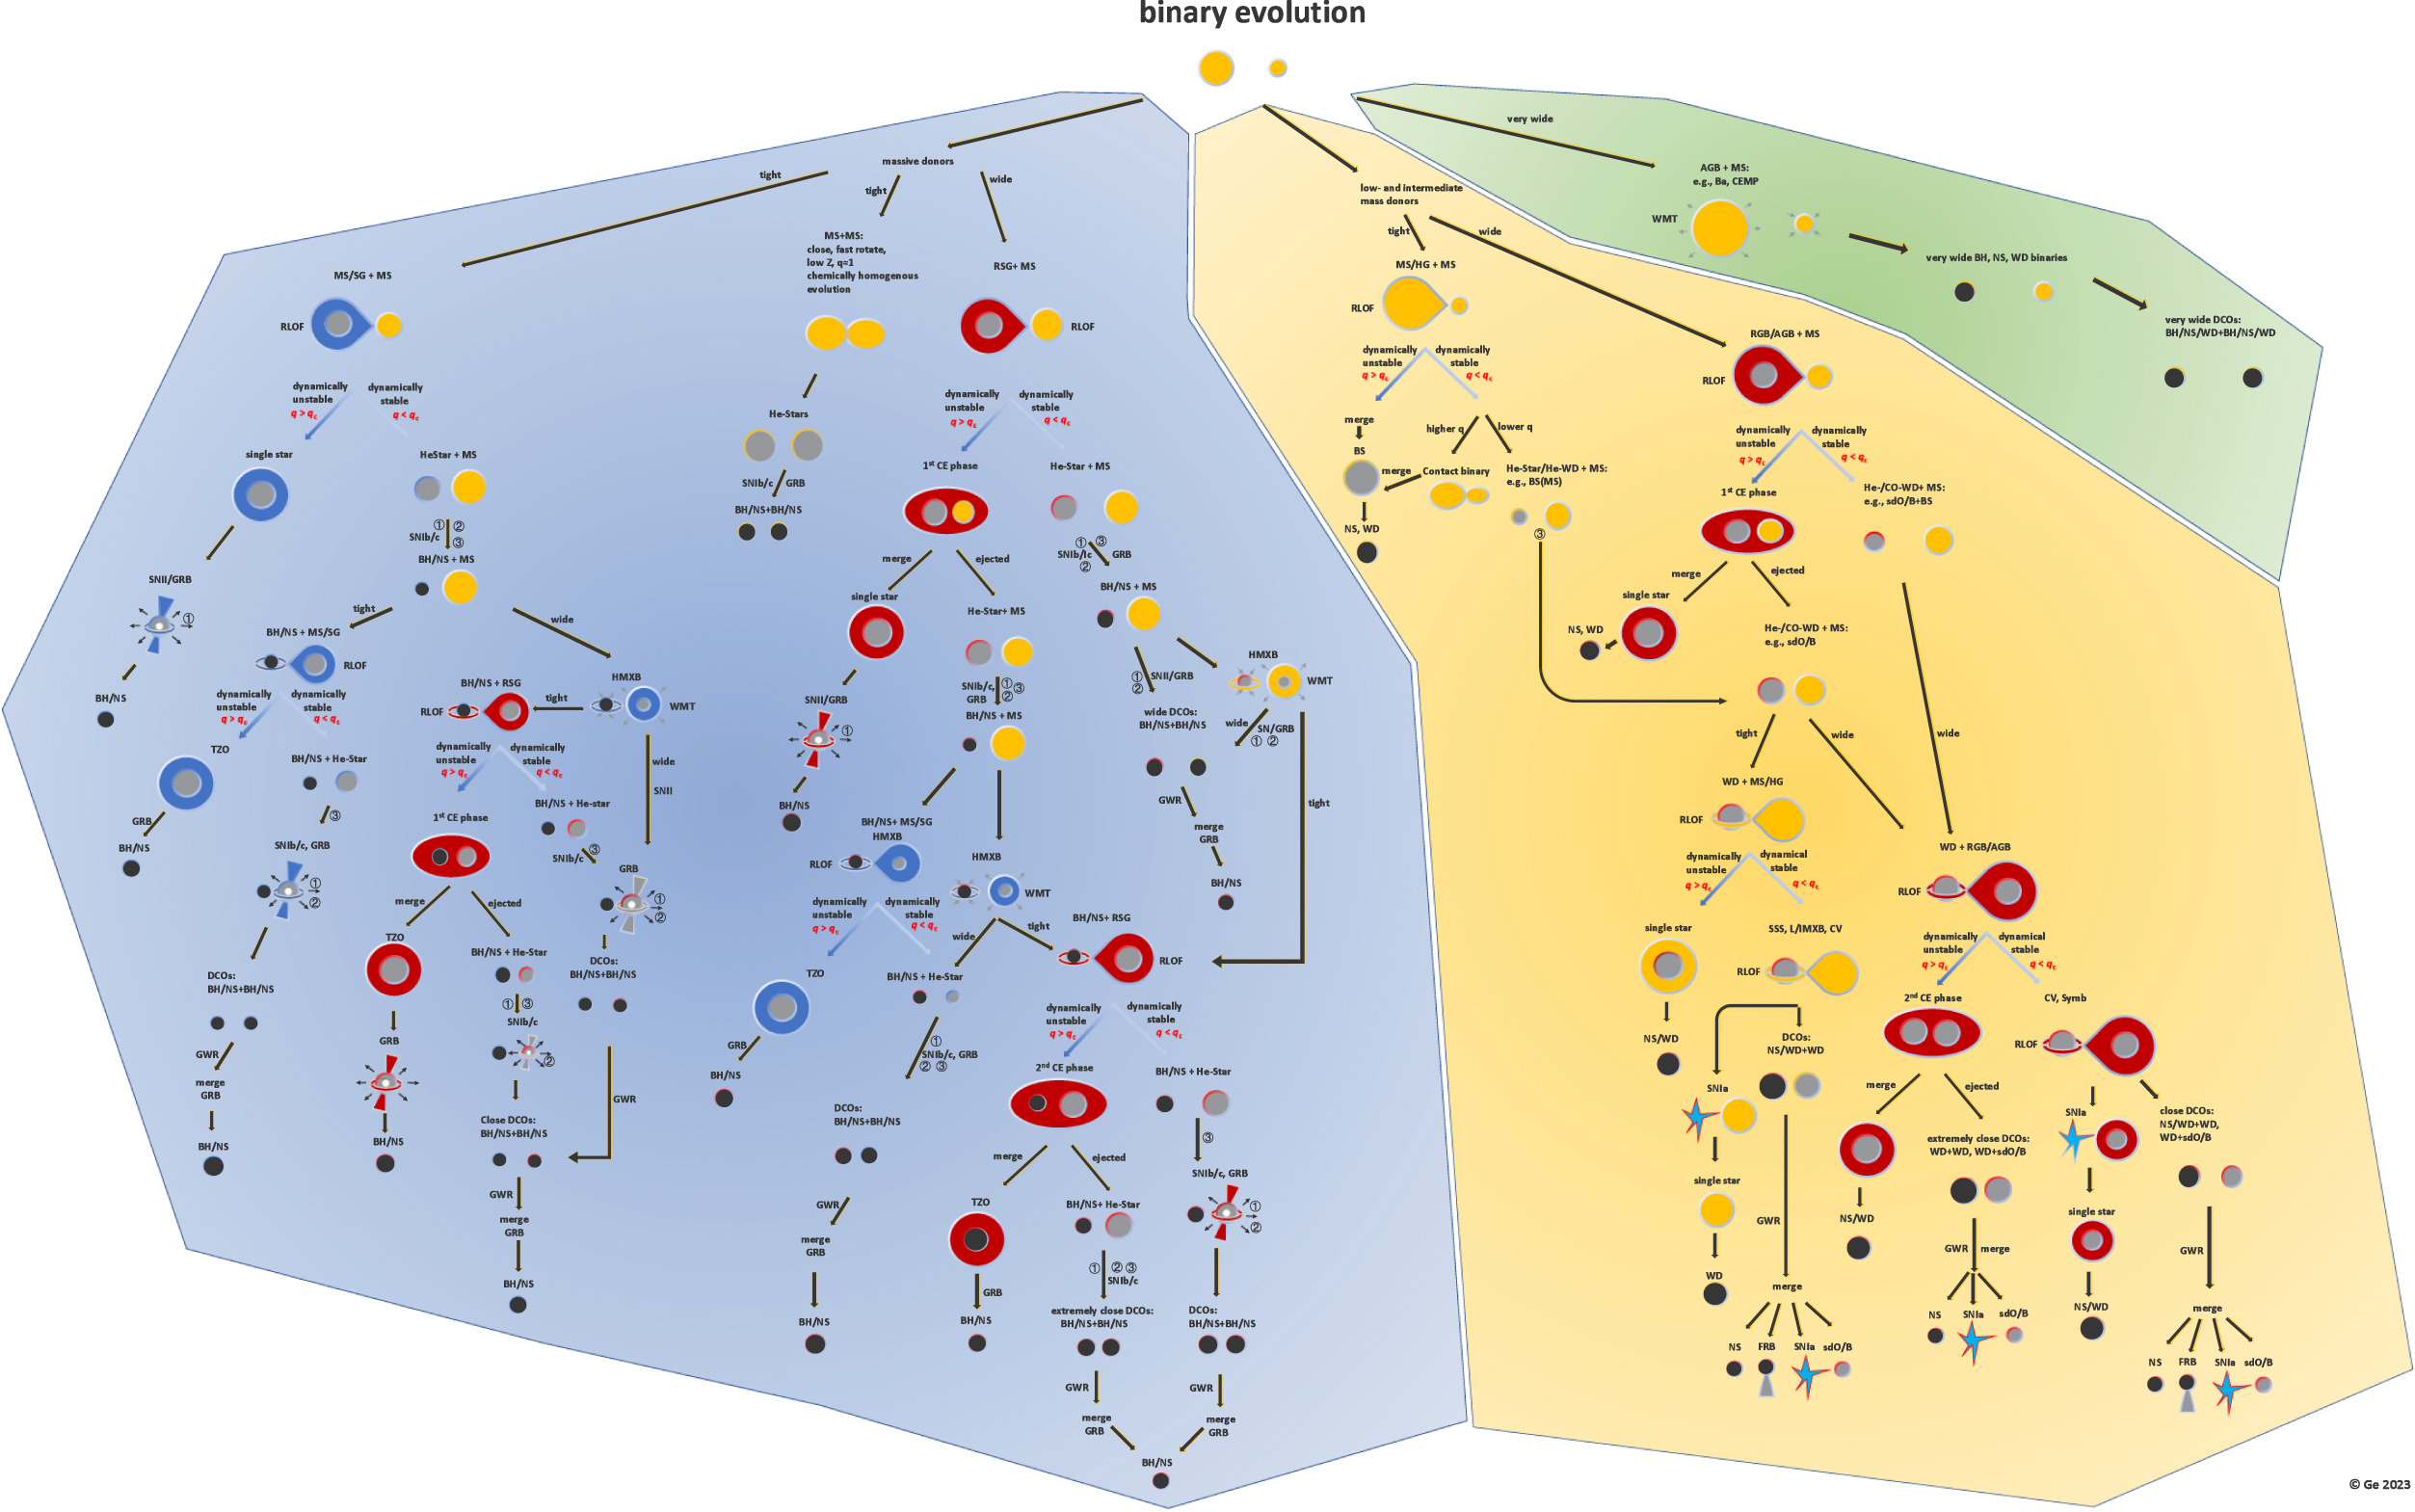
\includegraphics[width=\textwidth]{figs/Binary Evolution Flowchart.jpg}
        \caption{A comprehensive flowchart of various outcomes of binary systems in regard to masses and orbital separations.}
        \label{fig:binary_evolution_flowchart}
        \textit{\small Reprint from \cite{Chen_2024}}
    \end{figure}
    \vspace*{\fill}
    \restoregeometry

    \subsection{\centering Roche Lobe Model} % maybe find the orignal rlm paper and use that to elaborate? it feels weird to not talk more here about this, however, it would be very easy to just spend forever talking about it. 
        The Roche Lobe model was discovered by Édouard Roche (cite) and defines the gravitational potential of a binary through a simple model. Simply defined, it defines the region around a star where it can hold onto it mass (i.e. has great enough gravitational potential). If one of the stars in this binary \textit{exceeds} said lobe, it will transfer mass to its binary pair. This model can be used to classify binary star populations into various populations, including \textbf{Detached Binaries} (where neither star has filled their potential), \textbf{Contact Binaries} (where both stars have filled their potentials), and \textbf{Roche Lobe Overflow}(RLO) systems (where one star has filled its potential, leading to mass transfer to an accretor).
            

    \vspace*{\fill}
    \begin{figure}[h!]
        \centering
        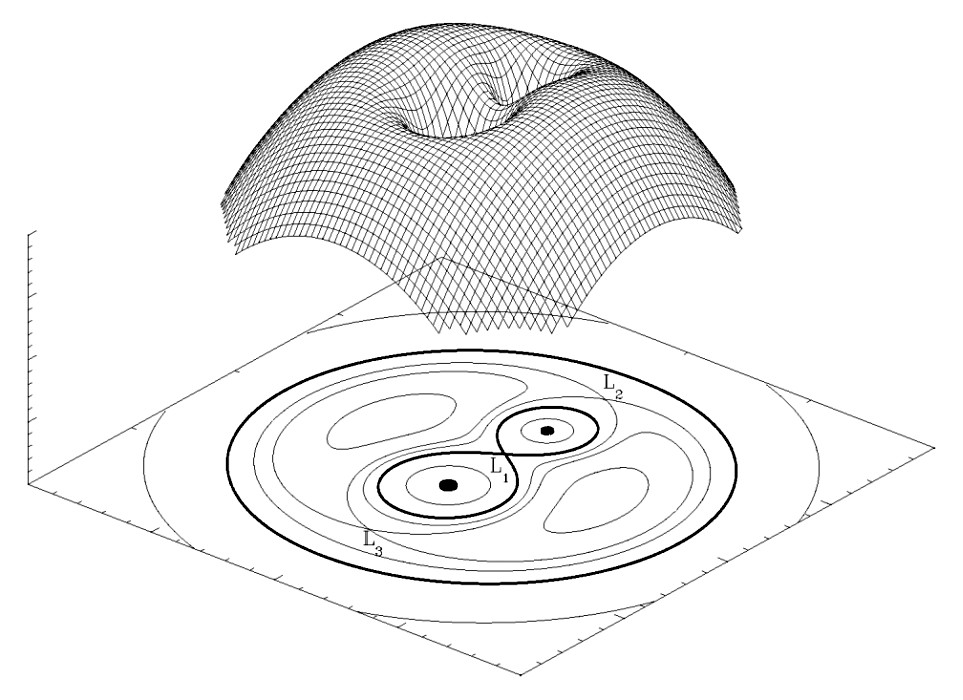
\includegraphics[width=\textwidth]{Figs/RochePotential.jpg}
        \caption{ A 3D representation of the gradient of the Roche lobe}
        \label{fig:Roche_potential}
        \textit{\small Reprint from \cite{TaurisvandenHeuvel+2023}}
    \end{figure}
    \vspace*{\fill}

        \subsection{\centering Detached}

        Systems where neither star fills its potential fully are called detached system. In these systems, two stars orbit a COM.

        However, in systems which are regarded as detached mass transfer is still possible through a processes called Wind Accretion (see \ref{WindAccretion}). We see this prominently in systems called \textit{High Mass X-ray Binaries}, where a supergiant star transfers mass to a compact object via wind accretion. This process leads to an increase in X-ray Emission, which we can measure.~\cite{TaurisvandenHeuvel+2023} It is important to note that these systems are not experiencing full-blown RLO, however, they tend to be incredibly close. \cite{TaurisvandenHeuvel+2023} These systems transfer mass through both wind accretion and in some cases, atmospheric Roche Lobe Overflow.

        I used the system Vela X-1 \cite{Kretschmar_2021} as an example of this, as it is generally regarded as the ``archetypical wind accretor''~\cite{Kretschmar_2021} 

        \subsubsection{Wind Accretion Mass Transfer} \label{WindAccretion}
        Wind accretion very different from normal mass transfer in a binary. All stars produce `wind', i.e. mass which is pushed away from the star. This process is called stellar winds, occurring when various types of mass is ejected at speed from the star. All stars have different processes of wind, with some have very high velocities of the wind, and others have lower velocities.~\cite{Lamers_1999} In binary stars this process can allow mass to be transferred from one star, to a generally smaller, accretor.
        
        
        \begin{figure}[h!]
            \centering
            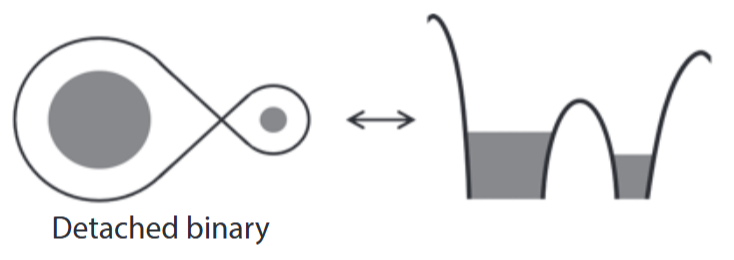
\includegraphics[scale = .4]{Figs/Detached binary.png}\\
            \textit{Reprint from~\cite{TaurisvandenHeuvel+2023}}
            \caption{Graphic of the RL model with regard to how much potential is being filled in a detached binary. Note here that has both a `top-down' perspective and from the side.}
            \label{DetachedBinaryRL}
        \end{figure}
        
        \subsection{\centering Roche Lobe overflow} % maybe include equations??
        In systems where one star fills its gravitational potential mass begins to be transferred to its binary partner. This is called Roche Lobe Overflow (RLO) and is defined by a donor and accretor star. 
        
        This is incredibly likely to happen at some point in a binaries' lifespan, and it will drastically affect its evolution~\cite{Chen_2024}. Depending on the systems star types, masses, and  eccentricity, this process will either be stable or unstable. When this process if unstable, it leads to either the common envelope, which results in either a merger or separation once more. However, if the process of mass transfer is stable, the two stars will remain detached.~\cite{Chen_2024}

        In this process, the mass will be transferred through the Lagrange point $L_1$, as it is the point of lowest potential between them, as seen in figure~\ref{fig:Roche_potential}. \cite{TaurisvandenHeuvel+2023}

        We are able to observe this commonly in X-ray Binaries, where a donor star transferred mass to an accretor which is a compact object (BH or NS). This process then produces X-rays which we can measure to understand the processes within the binary in greater detail.
        
       \begin{figure}[h] 
            \centering
            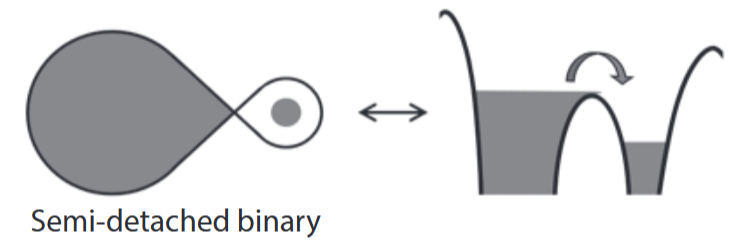
\includegraphics[scale = .4]{Figs/Semi-detached binary.png}
            \caption{\textit{Reprint from~\cite{TaurisvandenHeuvel+2023}}}
            \label{SemidetachedRL}
        \end{figure}
        
        I used the system V404 Cyngi with data from \cite{Bernardini_2016} and \cite{Shahbaz_1994} as an example of this behavior. 

        \subsection{\centering Contact Binary}
        In binaries where RLOF occurs it is possible for a star to fill up not just its potential, but the others as well. In cases like these the star then begins to fill up the binaries potential.\ (i.e.\ the area above the dark section in figure~\ref{ContactBinaryRL}) The system also has a limited potential, and if that fills as well, the system undergoes a stage called ``common envelope''


        This process generally is not stable, as most stars in stage generally are experiencing a stage of their evolution called common envelope (CE). (See section~\ref{CommonEnvelope}) However, in cases where it is stable, the stars evolve at the same rate, something called ``homogenous chemical evolution''. (See fig~\ref{fig:binary_evolution_flowchart}) Contact binaries generally have very little to no eccentricity, as their close orbits self stabilize.~\cite{TaurisvandenHeuvel+2023}
        
        \begin{figure}  
            \centering
            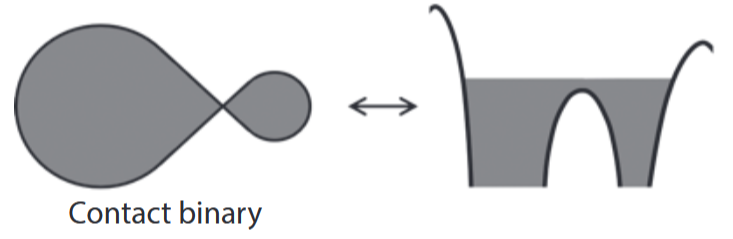
\includegraphics[scale = .4]{Figs/Conact Binary.png}

            \caption{\textit{Reprint from~\cite{TaurisvandenHeuvel+2023}}}
            \label{ContactBinaryRL}
        \end{figure}
        
        \subsubsection{Common Envelope}\label{CommonEnvelope}
            In the CE stage of binary evolution there are two distinct outcomes, both of which heavily depend on the systems initial conditions. These are that the two stars merge, becoming a single star, or that one star is ejected. 

            In this process the potential of the systems is completely filled, at which point mass stars being pushed out of the system through $L_2$. This mass then begins to form a pseudo disk around the stars, orbiting a slower rate~\cite{TaurisvandenHeuvel+2023}. This leads to be  This mass may be fully ejected from the system entirely, creating ionized gas around the stars,~\cite{TaurisvandenHeuvel+2023}which can be observed from earth. 

        \subsubsection{Stable Evolution}\label{StableEvoluton}
            In systems where mass transfer is not happening and both of the stars are at stable points in their evolution (i.e. both MS), the stars will share their mass. This means that their ``shells'' will evolve in tandem.

        I used W Ursae Majoris (W UMa) as an example of these systems, as it is used an example system in order to categorize these contact binaries as a whole.
    \subsection{X-ray Binaries} 
        \subsubsection{X-rays in accretion} \label{XrayAccretion}
        \subsubsection{Low Mass X-ray Binaries (LMXBS)} \label{lmxbs}
        \subsubsection{High Mass X-ray Binaries (HMXBS)} \label{Hmxbs}

        
        
        % \subsection{\centering X-ray Binaries}
        % In binaries with compact objects accretors (BHs and WDs) we find a large amount of produced X-ray binaries. We see this as bright Xray sources in our skies (cite). These X-rays are produced through mass falling into the accretor, causing xrays. (cite)
        
\section{\centering Data Acquisition}
    \subsection{\centering Vela X-1 (Detached)}
    
    \begin{table}
            \subsubsection{Known properties}
            \begin{center}
                \begin{tabular}{||c | c  c||} 
                 \hline
                 & Vela X-1 A & Vela X-1 B  \\ 
                 \hline\hline
                 \textbf{Star Type} & Neutron Star & Supergiant \cite{Kretschmar_2021} \\ 
                 \hline
                 \textbf{Masses}\(M_\odot\) & $\ge$ 1.8 \cite{Kretschmar_2021} & 20–30 \cite{Kretschmar_2021} \\
                 \hline
                 \textbf{Radius} & 11-12.5$_{KM}$ \cite{Kretschmar_2021} & 30 \(R_\odot\)
                 \cite{Kretschmar_2021} \\ % note that the stars are not spherical
                 \hline 
                 \textbf{Separation} &  \multicolumn{2}{c||}{2$kpc$ \cite{Kretschmar_2021}} \\
                 \hline 
                 \textbf{Mass Loss Rate} & \multicolumn{2}{c||}{$10^{-6} M_\odot yr^{-1}$ \cite{Kretschmar_2021}} \\
                 \hline
                 \textbf{Eccentricity} & \multicolumn{2}{c||}{$ e \approx  0.0898)$ \cite{Kretschmar_2021}} \\
                 \hline
                \end{tabular}
                \caption{Properties of Vela X-1} 
                \label{VelaX1} 
            \end{center}
    \end{table}

        Vela X-1 consists of a Neutron Star and Supergiant and is an Eclipsing and pulsing HMXB (sect. \ref{Hmxbs}). This means that the Neutron star passed behind the Supergiant every 8.94 days \cite{Falanga_2015}, leading to a variable luminosity between $10^{36}$ $erg$ $s^{-1}$ and $10^{37}$ $erg$ $s^{-1}$. Additionally, the neutron star itself is spinning every 293 seconds. \cite{Kretschmar_2021}. 
        
        Vela X-1 is described as an archetypical wind accretor, as it is a system which is undergoing wind accretion in a stable, predictable, and easy to measure way. The x-ray emission is persistent as well its broadband spectra. Astronomers use Vela X-1 as examples when looking at other systems with comparable x-ray emissions. \cite{Kretschmar_2021}
        
        The wind accretion (see \ref{WindAccretion}) comes in the form of wind from supergiant star (Vela X-1B) falling onto the neutron star. This wind does not have a very high velocity, but because the supergiant has almost filled it RL \cite{Kretschmar_2021}, the wind mass can easily escape, falling onto the NS. This accretion process (Sect. \ref{XrayAccretion}) is what creates the prominent X-ray emission.

        \subsubsection{Notes}   
            Vela X-1A has a mass defined to be higher than the Chandrasekar limit, which allows it to be used to help create models for compact stars and equations-of-state. \cite{Kretschmar_2021}
        
    \subsection{\centering W Ursae Majoris (Contact Binary)}
        \subsubsection{Known properties}

        \begin{table} 

            \begin{center}
                \begin{tabular}{||c | c c||} 
                    \hline
                    & W UMa A & W UMa B \\ 
                    \hline\hline
                    \textbf{Star Type} & O-Type \cite{Antokhina_2011} & O-Type \cite{Antokhina_2011} \\ 
                    \hline
                    \textbf{Masses}\(M_\odot\) & $1.139 ± 0.019$\cite{Gazeas_2021} & 0.551 ± 0.006\cite{Gazeas_2021} \\
                    \hline
                    \textbf{Radius}\(R_\odot\) & 1.092 ± 0.016\cite{Gazeas_2021} & 0.792 ± 0.015\cite{Gazeas_2021} \\
                    \hline
                    \textbf{Temperature}$K$ & 33750 \cite{Antokhina_2011}  & 33500 \cite{Antokhina_2011} \\
                    \hline
                    \textbf{Luminosity}\(L_\odot\) & 1.557 ± 0.166\cite{Gazeas_2021} & 0.978 ± 0.071\cite{Gazeas_2021}   \\ 
                    \hline
                    \textbf{Distance} & \multicolumn{2}{c||}{52$pc$ \cite{GaiaCollab_2018}}\\
                    \hline
                    \textbf{Max Magnitude} & \multicolumn{2}{c||}{7.75 \cite{Malkov_2006}} \\
                    \hline
                    \textbf{Min Magnitude} & \multicolumn{2}{c||}{8.48 \cite{Malkov_2006}} \\
                    \hline
                    \textbf{Period} & \multicolumn{2}{c||}{.3336 $days$ \cite{Gazeas_2021}}\\
                    \hline
                    \textbf{Inclination Plane}  & \multicolumn{2}{c ||}{$88.4 \pm 0.8^\circ$ \cite{Gazeas_2021}} \\
                    \hline
                \end{tabular}
                \caption{Properties of W Ursae Majoris} 
                \label{WUmaTable} 
            \end{center}
        \end{table}

        
        W UMa is a contact binary, meaning that the two stars are physically `connected' by their mass. This system is known as an archetype because is it has a high magnitude at 7.75 at peak and 8.48 at minimum (table \ref{WUmaTable}), meaning that its fairly easy to observe the variability. We can measure said variability in the form of light curves, which reveal a distinct nature different which is different from non-contact binaries (fig. \ref{WUMaLightcruve}). This magnitude variability is due to the fact that the binary is eclipsing due to its low inclination plane (table \ref{WUmaTable}), meaning that one of the stars will pass behind the other in its orbit relative to the Earth. 

        Because of the prominent nature of this binary, similar contact binaries are called referred to as `UWMa type' if they also possess said eclipsing nature. 

        \begin{figure}[h!]
            \centering
            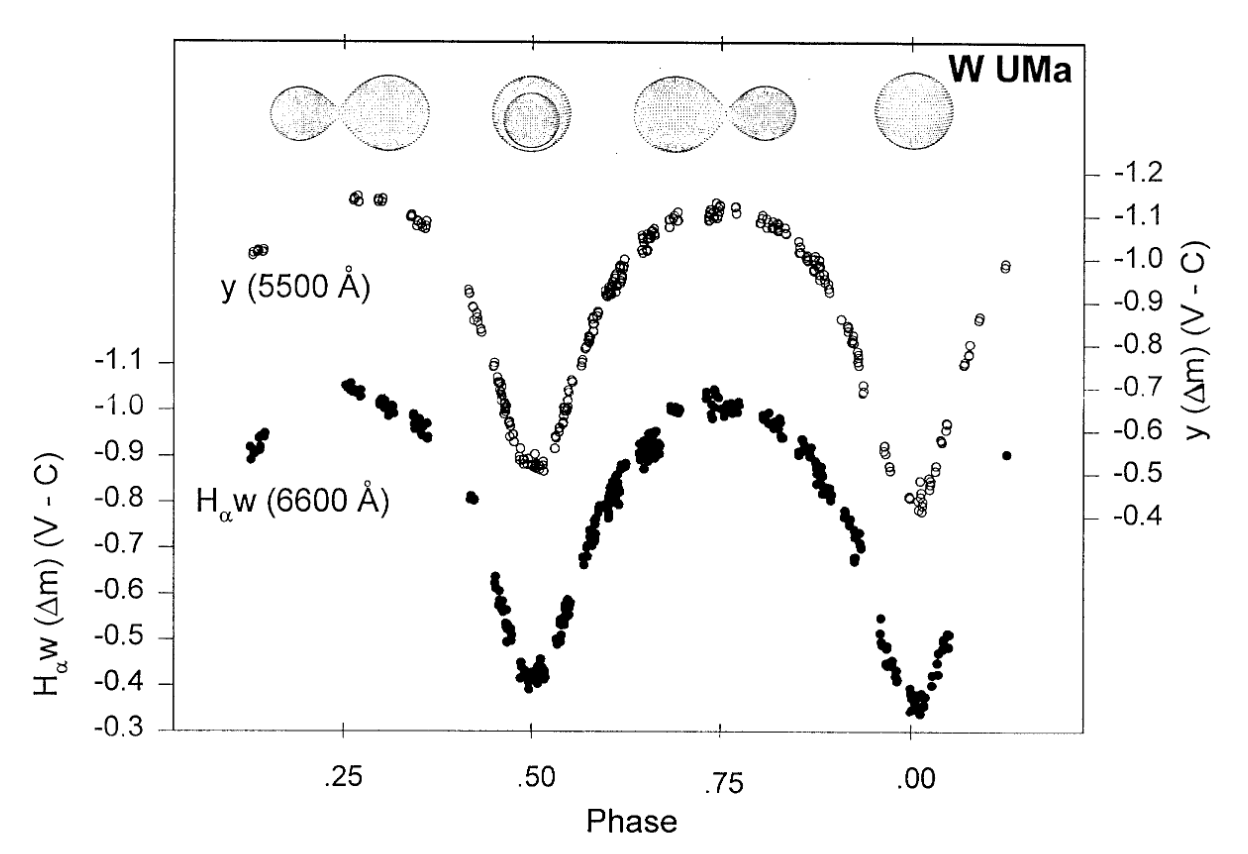
\includegraphics[scale= .3]{figs/W Uma Lightcurve.png}
            \caption{\textit{Reprint from~\cite{Morgan_1997}}}
            \label{WUMaLightcruve}
        \end{figure}
        \pagebreak

        % \subsubsection{Simulated}
        % Simulated data is good because of xyz and is useful because of xyz. data was made using xyz

    \subsection{\centering Roche Lobe overflow in V404 Cyngi}
        \subsubsection{Known properties}
        \begin{table}
            \begin{center} 
                \begin{tabular}{||c | c c||} 
                 \hline
                 & \textbf{V404 Cyngi B (Donor)} & \textbf{V404 Cyngi A (Black Hole)} \\ 
                 \hline\hline
                 \textbf{Star Type} & Early K-type Giant & Black Hole \\ 
                 \hline
                 \textbf{Masses}& $.7_{M_\odot}$ \cite{Bernardini_2016} & $9_{M_\odot}$ \cite{Shahbaz_1994} \\
                 \hline
                 \textbf{Radius} & $6.0_{R_\odot}$ \cite{Shahbaz_1994} &  \\
                 \hline
                 \textbf{Temperature} & $4800_K$ \cite{Shahbaz_1994} & \\
                 \hline
                 \textbf{Luminosity} & $10.2_{L_\odot}$ \cite{Shahbaz_1994} &  \\ 
                 \hline
                 \textbf{Distance} & \multicolumn{2}{c||}{$2390_{pc}$ \cite{Bernardini_2016}} \\
                 \hline
            \end{tabular}
            \caption{Properties of V404 Cygni} 
            \label{V404Data} 
            \end{center}
        \end{table}

        V404 is a LMXB (sect \ref{lmxbs}), meaning that the donor star has a relatively low mass, generally $\leq 1 M_\odot$ \cite{Bahramian_2023}. In this system the material being accreted by V404 Cyngi A forms an accretion disk, greatly increasing the luminosity of the system.

    \subsection{POSYDON Simulations}
         I used data generated by POSYDON \cite{Fragos_2023} in corroboration with three observed systems in order to fully understand the depth of the process of mass transfer in Binary Systems. This is because while catalogues of contact binaries, HMXBs and LMXBs exist, there is not enough of them to get a true grasp of the full picture. Hence, I used POSYDON. This dataset was simulated on the NU Super computing Cluster, QUEST. POSYDON is developed and maintained by a team of astrophysicists and computer scientists working at the Université de Genève and Northwestern University. POSYDON uses an additional script called MESA, which is dedicated to single star and binary evolution. POSYDON utilities MESA on a much larger scale in order to simulate full populations. The data was stored in the form of a .h5 file, containing a total of $approx$6.1 million rows and 83 columns. (See greatly reduced example of the data frame in (table \ref{POSYDONDataExample}) and an HR Diagram of the full dataset in Fig. 2)

         \begin{table}[h]
            \centering\
            \footnotesize
            \begin{tabularx}{\textwidth}{||X | X | X | X | X | X | X | X ||}
                \hline
                \textbf{Binary ID} & 
                \textbf{System State} & 
                \textbf{Orbital Period (days)} & 
                \boldmath$\log_{10}$ \textbf{Mass Transfer Rate} & 
                \textbf{Donor State} & 
                \textbf{Donor Mass} $M_\odot$ & 
                \textbf{Accretor State} & 
                \textbf{Accretor Mass} $M_\odot$
                \\ \hline
                $54$ & Detached & $0.047520$ & $-99.00000$ & NS & $1.196033$ & stripped He Core He burning & $\approx 1.002$ \\
                \hline
                $183$ & Detached & $0.0429883$ & $ \approx -80.8$ & NS & $1.196033$ & stripped He Core He burning & $\approx .9957$ \\
                \hline
            \end{tabularx}
            \caption{Example of POSYDON data, heavily modified for readability}
            \label{POSYDONDataExample}
        \end{table}

        \begin{figure} [h]
            \centering
            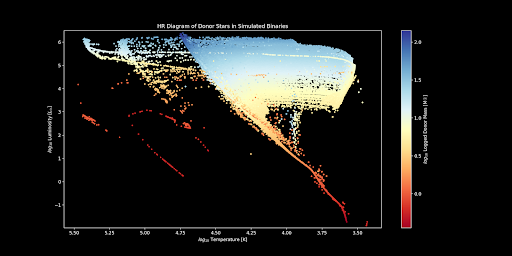
\includegraphics[width = \textwidth]{figs/EntireDataSetHR.png}
            \caption{HR Diagram of the donor star for the full POSYDON dataset. Note that the color of the plotted points correspond to the $log_{10}$ mass of the donor star. Generated with Matplotlib}
        \end{figure}
        \pagebreak

\section{\centering Results}
    With my research I sought to contextualize these very specific systems, allowing one to better understand how these systems play into the larger picture of binaries in
    
        \subsection{\centering Detached}
        In detached binaries, there is still the possibility for mass transfer. These systems are typically called HMXBs. I found that these systems have a distribution as pictured. Note these systems are only ones with full-blown RLO due to simulation of WA constraints
        \begin{center}
            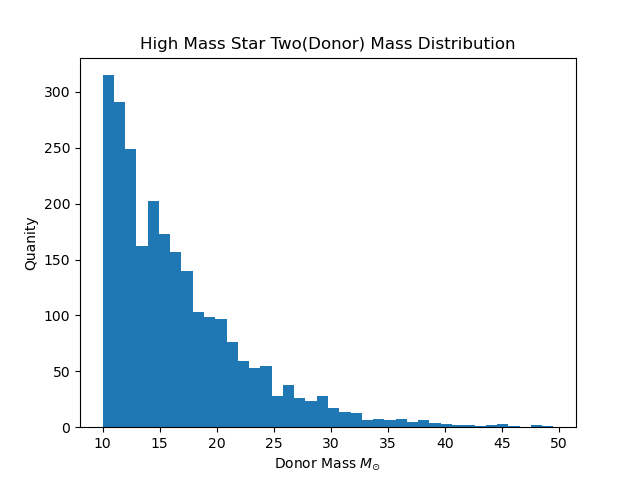
\includegraphics[scale = .6]{Figs/High Max X-ray Binary Star Two Mass Distro.png}
            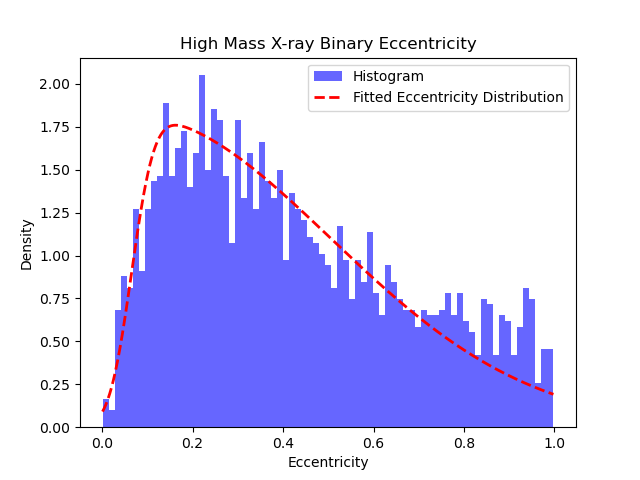
\includegraphics[scale =.6]{Figs/High Mass X-ray Binary Eccentricity.png}
        \end{center}
        Additionally, HMXBs fall in this region on the HR diagram 
        \begin{center}
            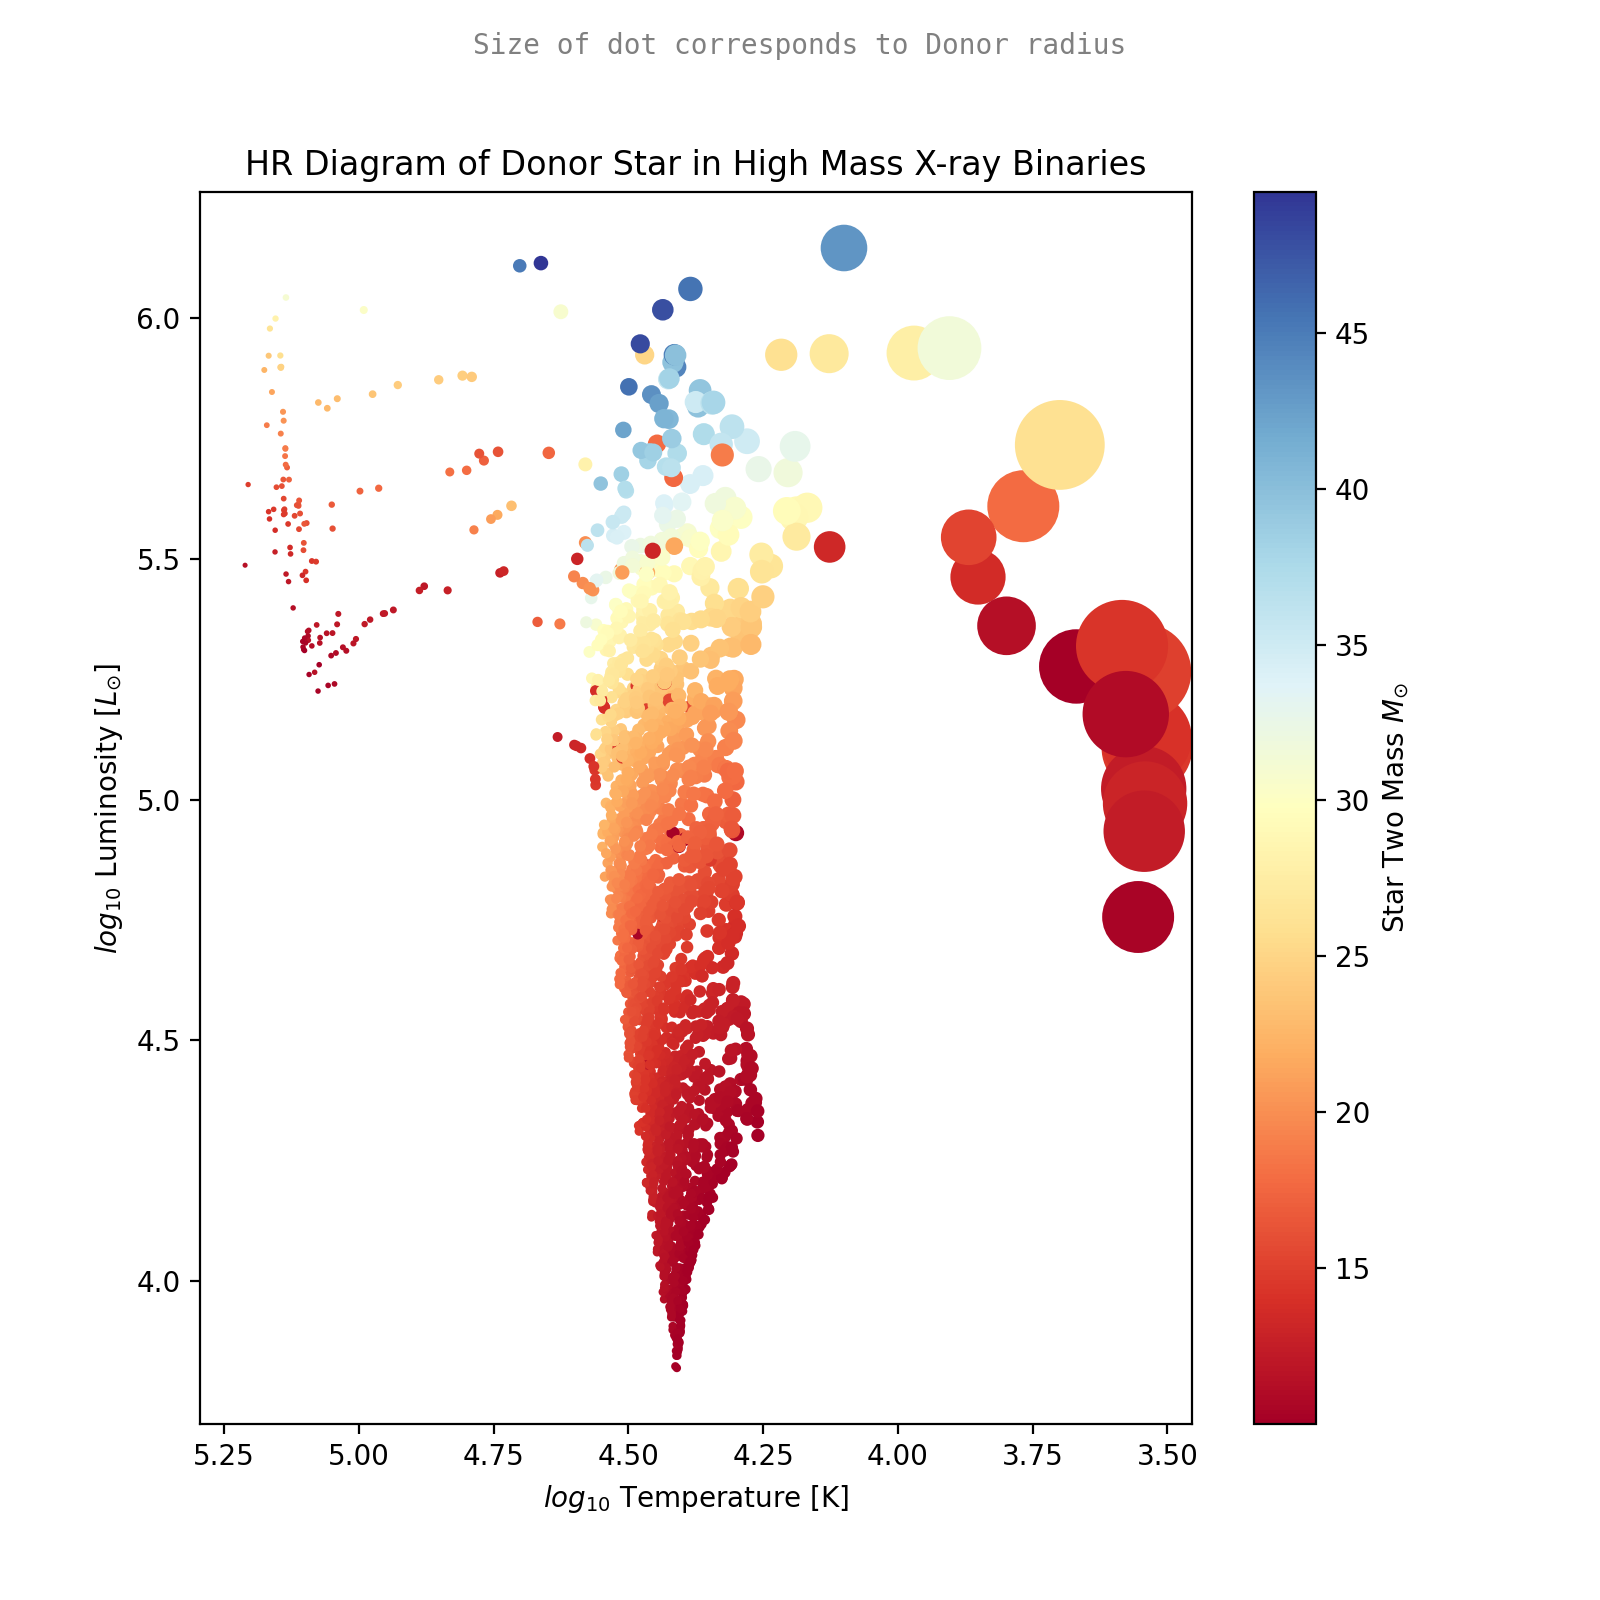
\includegraphics[scale = .5]{Figs/HR Diagram of Donor Star in High Mass Xray Binaries S2mass log10 F star radius T (2).png}
        \end{center}
  
        \subsection{\centering Roche Lobe Overflow}
        Full-blown RLO occurs in both all types of XrB's, including both HMXBs and LMXBs. These systems 
        \begin{center}
            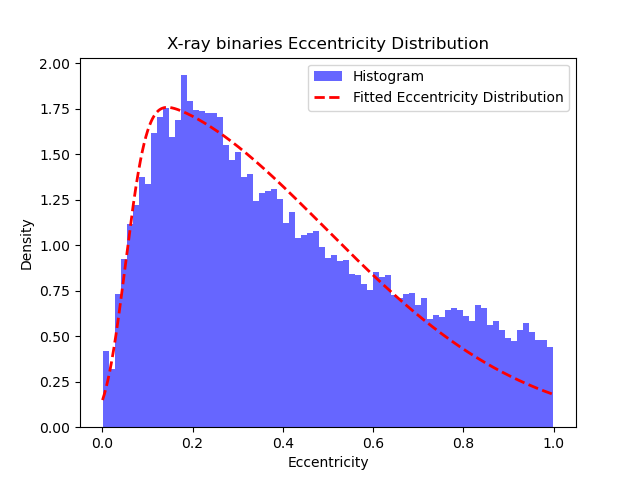
\includegraphics[scale=.5]{Figs/X-ray binaries Eccentricty Distribution.png}
            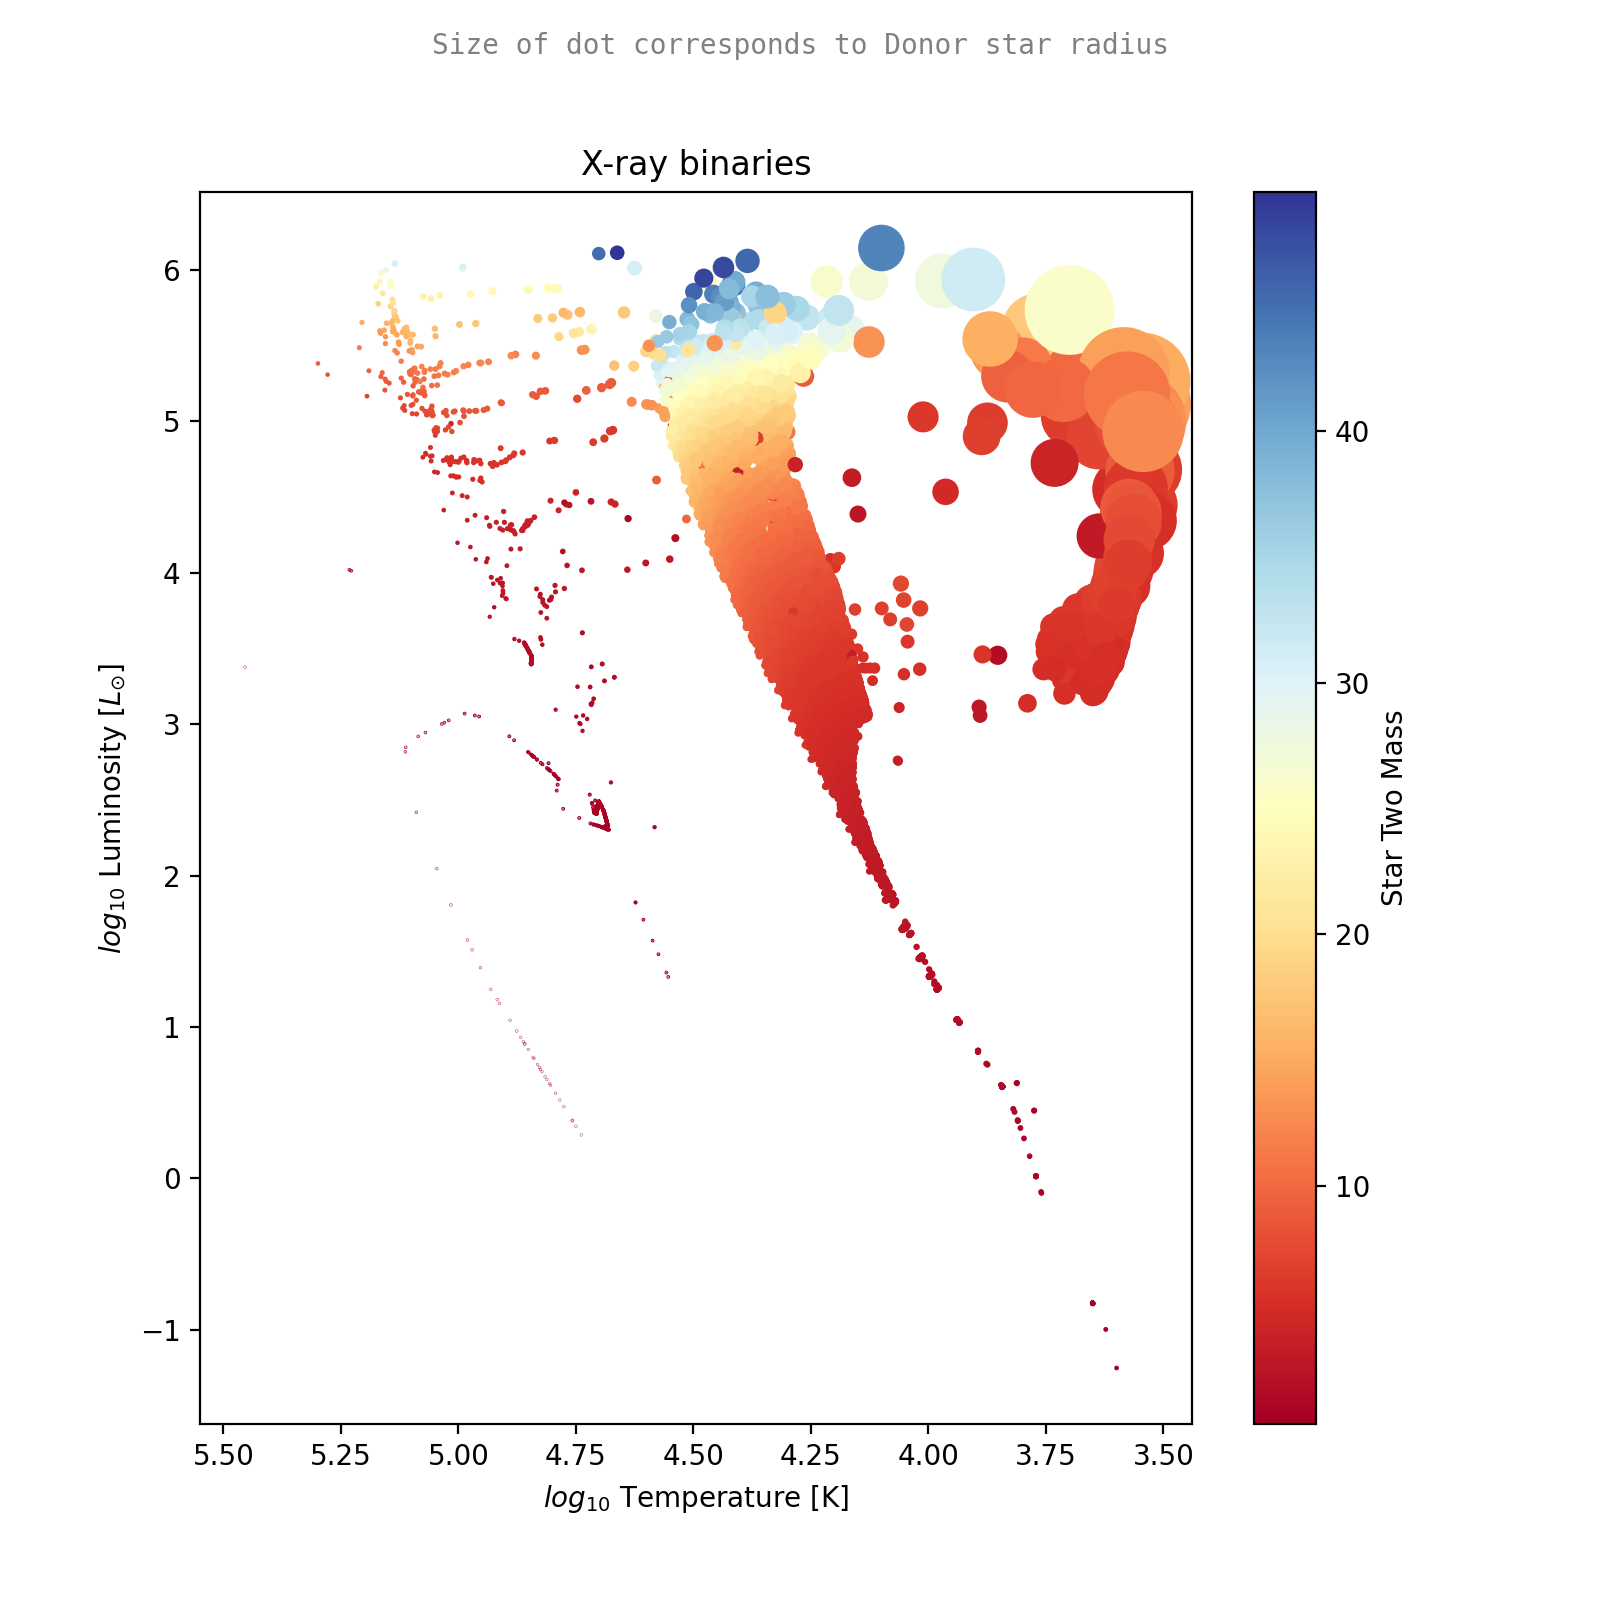
\includegraphics[scale=.5]{Figs/X-ray binaries S2mass log10 F star radius T.png}
            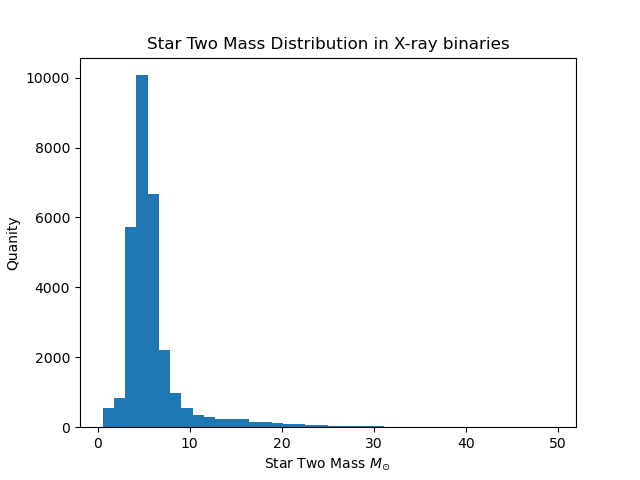
\includegraphics[scale=.6]{Figs/X-ray binaries Star Two Mass Distribution.png}
            
        \end{center}
        (cite and insert figs)
      
        \subsection{\centering Contact Binary}
        I found that in CE systems this can happen with these evolutionary changes. We see an example in observed systems (insert source and figs) in our POSYDON \cite{Fragos_2023} simulated data too. (figs)

        \begin{center}
            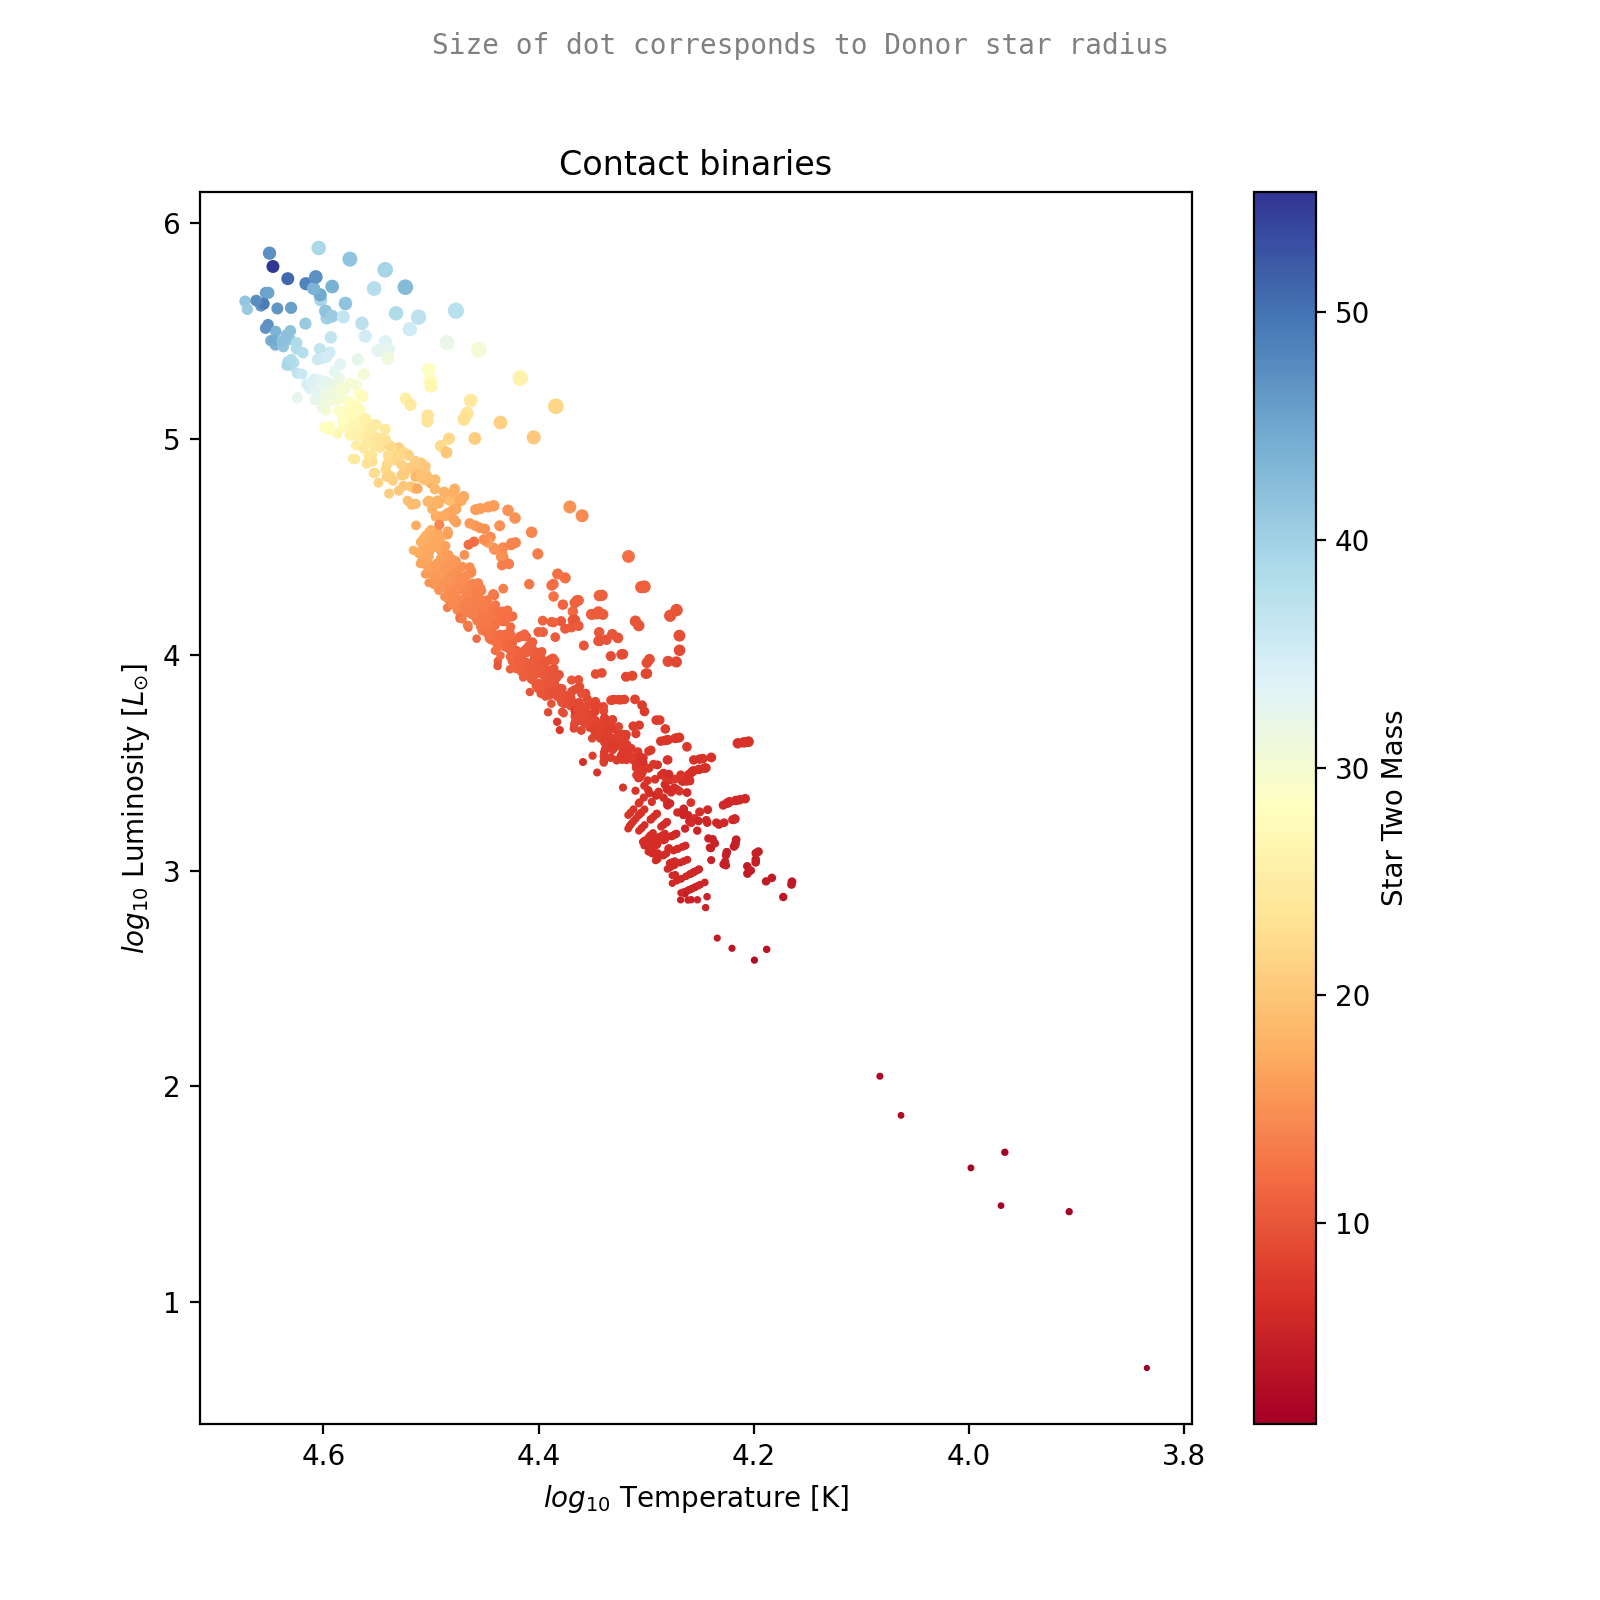
\includegraphics[scale = .6 ]{Figs/contact binary HR diagram.png}
            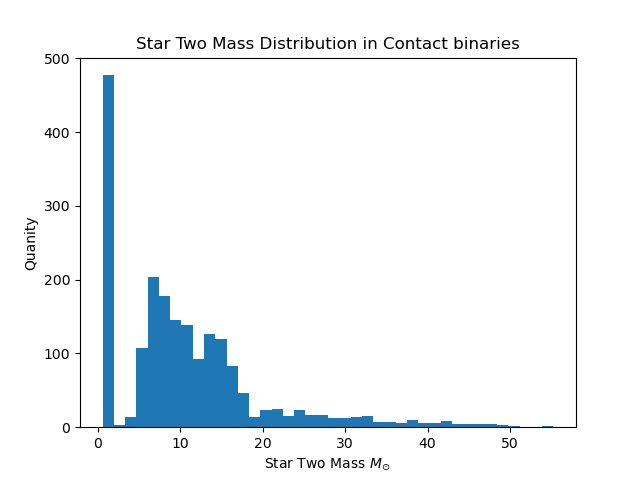
\includegraphics[scale = .5 ]{Figs/Contact binaries Star Two Mass Distribution.png}
        \end{center}
    % \subsection{\centering ii) Type 1a Supernova}
    % I found that in systems with type 1a SN the progenitors tend to be ..., this is corroborated with this paper (cite). We see a similarity with the POSYDON data and this papers data
 
    % \subsection{\centering iii) X-Ray Binaries}
    % I found that XrBs mass transfer effects them by causing changes to ... we see this our POSYDON data and this paper... 

\section{\centering Discussion}   
    Originally I planned on simulating grids for all the types of systems, however, due to time constraints I chose to only focus on one type. 

    \subsection{Git Galore}
    Originally, I started working on this project using Overleaf, however, due the amount of graphs, the time to compile started to rapidly climb up, and eventually I just decided to switch to compiling it locally. On-top of this, I figured I would set up a GitHub in order to additionally push the code and graphs as well. This turned out to absolutely be the right decision, giving me way more freedom.
    
\section{\centering Conclusion}
    In conclusion mass transfer effects binary systems in these ways, which can lead to these evolutionary outcomes. 

\printbibliography[
heading=bibintoc,
title={\centering Sources}
]

\end{document}